\begin{frame}
    \frametitle{EJERCICIOS RESUELTOS DE RAZONES}


\begin{enumerate}
\item En un curso, la razón entre la cantidad de hombres y de mujeres es 3 : 2. Si hay 24 hombres, ¿cuántos estudiantes hay en 
total en el curso?

\hfill

{\small
Respuesta: Hay 40 estudiantes en el curso, 24 hombres y 16 mujeres.
}

\item Un gásfiter y su ayudante, reciben por la instalación de tres sanitarios \$ 270.000, los que se reparten en la razón 7 : 
2, 
¿cuánto dinero recibirá cada uno?

\hfill

{\small
Respuesta: Pago al ayudante: \$ 60.000  Pago del gásfiter: \$ 210.000
}
\end{enumerate}

\end{frame}

\begin{frame}
    \frametitle{EJERCICIOS RESUELTOS DE RAZONES}


\begin{enumerate}

\item El perímetro de una cancha de fútbol mide 432 metros. Si la razón entre el ancho y el 
largo es 5:7. ¿cuánto mide cada lado de la cancha?

\hfill

{\small
Respuesta: El ancho de la cancha es de 90 metros y el largo 126 metros.
}

\item Las medidas de los ángulos interiores de un triángulo están en la razón 4 : 15 : 17 ¿Cuánto mide cada uno de los 
ángulos?

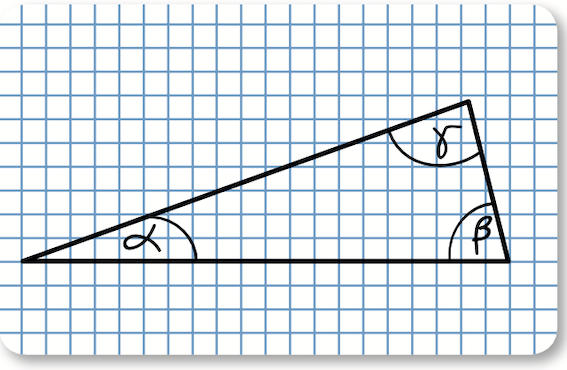
\includegraphics[scale=.3]{rectan}
\hfill

{\small
Respuesta: La medida de los ángulos interiores es $\alpha= 20^o, \beta = 75^o, \gamma= 85^o$
}

\end{enumerate}

\end{frame}
